\newpage
\chapter{Apache Spark} 

Apache Spark wurde ist ein Open Source Framework, dass ermöglicht Software verteilt \"uber ein Cluster auszuführen. Dar\"uber hinaus ist die Programmier-Modell mit Apache Spark sehr elegant und einfach gehalten. [\cite{AAWS15}] \\
Im Rahmen eine Forschungsprojekts ist Apache Spark entstanden. Das Forschungsprojekt wurde 2009 in der Universtiy of California in Berkeley im sogenannten AMPLab\footnote{AMPLab: Todo} ins Leben gerufen. Seit 2010 steht es als Open Source Software unter der BSD-Lizenz \footnote{BSD-Lizenz (Berkeley Software Distribution-Lizenz): bezeichnet eine Gruppe von Lizenzen, die eine breitere Wiederverwertung erlaubt.} zur Verfügung. Das Projekt wird seit 2013 von der Apache Software Foundation\footnote{Apache Software Foundation: TODO} weitergef\"uhrt. Seit 2014 ist es dort als Top Level Projekt eingestuft. Zum aktuellen Zeitpunkt steht Apache Spark unter der Apache 2.0 Lizenz\footnote{Apache 2.0 Lizenz: Die Software darf frei verwendet und ver\"andert werden. Zus\"atzlich gibt es nur wenige Auflagen.} zur Verf\"ugung. \\
Der Code liegt auf GitHub\footnote{GitHub: Todo } und ist f\"ur jeden zug\"anglich. Bis zum 10.04.2017 gab es bereits 51 Releases, 19,365 commits und 1,053 contributors\footnote{contributors: Todo }.

% \ref{sec_sparkr} %\nameref{sec_sparkr} .

\section{Kern-Bibliotheken / Komponenten}

Apache Spark besteht im wesentlichen aus f\"unf Modulen: Spark Core, Spark SQL, Spark Streaming, MLlib Machine Learning Library und GraphX. 
Die Module werden in den folgenden Kapitel n\"aher beleuchtet. 
Dar\"uber hinaus wird in Kapitel \ref{sec_sparkr} noch eine weiteres interessantes Modul vorgestellt welches nicht direkt zum Kern geh\"ort, SparkR.
Die Aufteilung in die verschiedenen Module macht er sehr gut m\"oglich nur einen Teil der Module zu verwenden. 

\subsection{Grundlage des Systems (Spark-Core \& RDD’s)}\label{sec_sparkcore}

\newpage
\subsection{SQL-Abfragen mit (Spark-SQL \& Data Frames)}

Spark-SQL wurde 2014 veröffentlicht. Die Komponente gehört zu den Komponenten aus der Spark-Familie, die am meisten weiterentwickelt werden. 


Dabei kombiniert es zwei wesentliche Dinge. Zum einen ermöglicht es relationale Querys zu schreiben und zum anderen prozedurele Algorithmen einzusetzen. Bisher wurden beide Aktionen nacheinander von verschiedenen Systemen realisiert. 

SparkSQL entstammt dem Apache-Shark. Man wollte die Probleme die es in Apache Shark gab lösen.
\begin{enumerate}
	\item Mit Apache Shark ist es nur möglich auf Daten im Hive Katalog zuzugreifen. 
	\item Shark lässt sich nur über selbst geschriebene SQL's aufrufen. 
	\item Hive ist nur für MapReduce optimiert
\end{enumerate}

Mit ApacheSQL hat man erreicht auf relationale Daten zuzugreifen. Es wurde eine hohe Performance aufgrund etablierter DBMS-Techniken erreicht.
Neue Datenquellen lassen sich leicht anschließen und integrieren.
Zusätzliche Erweiterungen wie Maschine Learning und Graph Processing sind nutzbar.

Todo, auf Dataframe API eingehen.
Todo, auf Catalyst eingehen.


%eventuell in die Performance section
Gerade bei SQL ists es enorm wichtig sich für die richtigen Anweisungen zu entscheiden um keine langsamen Operationen zu haben. 
Hier gibt es sehr große Geschwindigkeitsunterschiede.

\newpage
\subsection{Verarbeitung von Datenströmen (Spark-Streaming)}

\subsection{Berechnungen auf Graphen (GraphX)}

\subsection{Maschinelles Lernen (MLlib)}

\subsection{Skalierung von R Programmen (SparkR)}\label{sec_sparkr}

\newpage
\section{Mehrere Komponenten im Verbund}

\newpage
\section{Performance}
%PAPER: Scaling Spark in the Real World
Analysen von Performance Probleme erweisen sich mitunter als sehr schwierig. Apache Spark bringt zwar die seiteneffektfreie API mit, jedoch kann trotzdem eine Menge schief gehen. Es ist schwer immer im Hinterkopf zu behalten, dass Operationen auf vielen verteilten Rechnern ablaufen. \\ \\
\"Uber eine Webbasierte Übersicht ist es Möglich Informationen zu dann aktuell laufenden Auswertungen und Dauer von Ergebnissen etc. zu bekommen. \footnote{Vgl. \cite[12]{AAWS15}}

Todo Beispiel Bild erstellen und erklären.
Es gibt ein Live-Dashboard.
Es gibt einen Stack-Trace Button




\subsection{Besonderheiten bei der Speichernutzung}
Zusätzlich wird oft unterschätzt, dass die Wahl einer geeigneten bzw. speichereffizienten Datenstruktur sehr viel bewirken kann.
Spark geht davon aus, eine Datei in Blöck einer bestimmten Größe geladen wird. In der Regel 128MB. Zu beachten ist jedoch, dass beim dekomprimieren größer Blöcke entstehen können. So können aus 128Mb schnell 3-4GB große Blöcke werden. \\ \\
Um das Speichermanagement zu verbessern wurde ein per-node allocator implementiert. Dieser verwaltet den Speicher auf einer Node. 
Der Speicher wir in drei Breiche geteilt. 
Speicher zum verarbeiten der Daten.  
Speicher für die hash-tables bei Joins oder Aggretaions
Speicher für \"unrolling\" Blöcke, um zu prüfen ob die einzulesenden Blöcke nach dem entpacken immer noch klein genug sind damit diese gecached werden können.\\ \\
Damit läuft das System robust über eine großen Bereich. 

\subsection{Netzwerk und I/O-Traffic}

Mit Spark wurde schon Operationen bei denen über 8000 Nodes involviert waren und über 1PB an Daten verarbeitet wurden durchgeführt.
Das beansprucht natürlich die I/O Schicht enorm. 


Um I/O Probleme zu vermeiden, bzw. diese besser in den Griff zu bekommen wurde als Basis das Netty-Framework\footnote{Netty: High-Performance Netzwerk Framework} verwendet.
\begin{itemize}
	\item Zero-copy I/O:\\
	Daten werden direkt von der Festplatte zu dem Socket kopiert. Das vermeidet Last an der CPU bei Kontextwechseln und entlastet zusätzlich den JVM\footnote{JVM: Todo} garbage collector\footnote{garbage collector: Todo}
	\item Off-heap network buffer management:\\
	Todo
	\item Mehrfache Verbindungen:\\
	Jeder Sparker worker kann mehrere Verbdingungen parallel bearbeiten.
\end{itemize}


\newpage
\section{Nutzung \& Verbreitung}

Durch die Unterstützung der drei Programmiersprachen skala, pathon und java ist arbeit mit Apache Spark einfacher, als wenn es nur einen einzige exotische Programmiersprache zur Nutzung gäbe. \\
Apache Spark unterstützt zudem noch verschiedene Datenquellen und Dateiformate.  Zu den Datenquellen zählen die das Dateisystem S3\footnote{S3: Todo} von Amazon und das HDFS\footnote{HDFS (Hadoop Distributed File System): Todo}.
Die Dateiformate können strukturiert (z.B.: CSV, Object Files), semi-strukturiert (z.B.: JSON) und unstrukturiert (z.B.: Textdatei) sein.


Unter den Mitwirkenden(Contributors) zählen über 400 Entwickler aus über 100 Unternehmen, Stand 2014 \\
Es gibt über 500 produktive Installationen. %PAPER: Scaling Spark in the Real World
%http://spark.apache.org/community.html
Seit einigen Jahren finden weltweit jährlich unter dem Namen Spark Summit Konferenzen statt.\\
%https://www.heise.de/developer/meldung/Big-Data-Umfrage-zur-Verbreitung-zu-Apache-Spark-2529126.html
Heise.de beauftrage 2015 eine Umfrage in der 2136 Teilnehmer befragt wurden. Diese gaben an, dass 31\% Prozent den Einsatz derzeit prüfen. 13\% Nutzen bereits Apache Spark und 20\% planten den Einsatz noch in dem damaligen Jahr.
Scala lag als Programmiersprache mit großen Abstand vorn. Die Nutzung innerhalb verschiedener Berufsgruppen war sehr ähnlich. Mit 16\%  lag bei den Telekommunikationsunternehmen der Einsatz am höchsten. Eine detaillierte Übersicht ist in \autoref{fig:nutzung} zu sehen.
\begin{figure}[h]
  \centering
  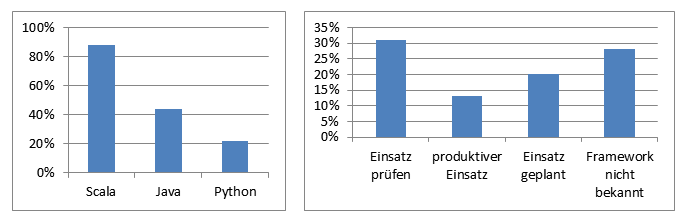
\includegraphics[width=\textwidth]{./excel/Nutzung.png}
  \caption{Einsatz \& Verbreitung}\label{fig:nutzung}
\end{figure}

%https://www.heise.de/developer/meldung/Big-Data-Umfrage-zur-Verbreitung-zu-Apache-Spark-2529126.html


